\documentclass[tikz,border=10pt]{standalone}

\begin{document}
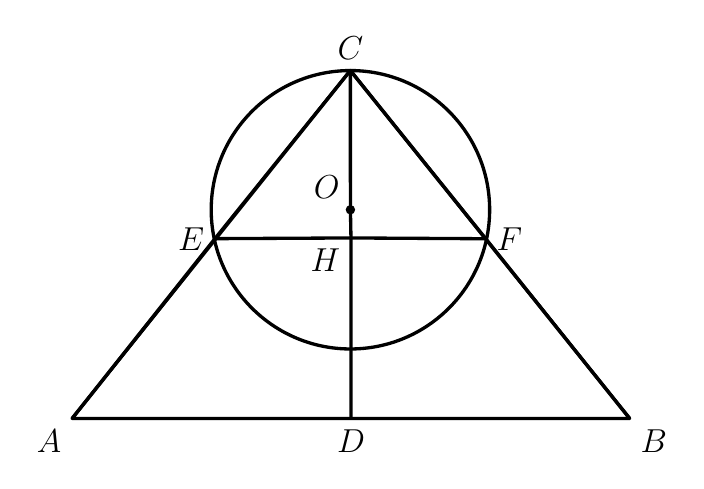
\begin{tikzpicture}[line width=1.2pt, line join=round, font=\fontsize{12}{14.4}\selectfont]
\coordinate (A) at (-3.556,-2.202);
\coordinate (B) at (3.524,-2.202);
\coordinate (C) at (-0.023,2.217);
\coordinate (D) at (-0.015,-2.202);
\coordinate (E) at (-1.743,0.081);
\coordinate (F) at (1.697,0.080);
\coordinate (H) at (-0.015,0.090);
\coordinate (O) at (-0.022,0.448);











  
  \draw (A) -- (B) -- (C) -- cycle;

  
  \draw (A) -- (E) -- (C);
  \draw (B) -- (F) -- (C);

  
  \draw (A) -- (D) -- (B);

  
  \draw (C) -- (O) -- (H) -- (D);

  
  \draw (E) -- (H) -- (F);

  
  \draw (O) circle[radius=1.768];

  
  \fill (O) circle[radius=0.060];

  
  \node[above] at (C) {$C$};
  \node[below left] at (A) {$A$};
  \node[below right] at (B) {$B$};
  \node[below] at (D) {$D$};
  \node[left] at (E) {$E$};
  \node[right] at (F) {$F$};
  \node[below left] at (H) {$H$};
  \node[above left] at (O) {$O$};

\end{tikzpicture}
\end{document}